\section{ Live Variabl Analysis   }

In compilers, live variable analysis (or simply liveness analysis)
 is a classic data-flow analysis to calculate the variables that 
 are live at each point in the program. A variable is live at 
 some point if it holds a value that may be needed in the future, 
 or equivalently if its value may be read before the next time 
 the variable is written to. \footnote{based on Wikipedia}

\subsection{Motivation}

Programs may contain 

\begin{itemize}
\item code which gets executed but which has no useful
effect on the program's overall result;
\item occurrences of variables being used before they
are defined;
\item many variables which need to be allocated
registers and/or memory locations for compilation.

\end{itemize}

The concept of variable liveness is useful in dealing 
with all three of these situations.



\subsection{Problem formulation}
Liveness is a data-flow property of variables:
“Is the value of this variable needed?” We therefore 
usually consider liveness from an instruction's 
perspective: each instruction (or node of the
flowgraph) has an associated set of live variables.


\subsection{Semantic vs. syntactic}

\footnote{based on slides from Cambridge University}


There are two kinds of variable liveness : Semantic liveness and Syntactic liveness.


A variable x is \textbf{semantically} live at a node n if there is
some execution sequence starting at n whose (externally
observable) behaviour can be affected by changing the
value of x. Semantic liveness is concerned with
the execution behaviour of the program.

A variable is \textbf{semantically} live at a node if there is a
path to the exit of the flow graph along which its
value may be used before it is redefined. Syntactic liveness is concerned with properties of
the syntactic structure of the program.


So what is the difference between Semantic liveness and Syntactic liveness? syntactic liveness
is a computable approximation of semantic liveness.


Consider the example 


\begin{lstlisting}[language=C,frame=single, caption=An ,label = lst:expr2]
    int t = x * y;
    if ((x+1)*(x+1) == y) {
     t = 1;
    }
    if (x*x + 2*x + 1 != y) {
     t = 2;
    }
    return t;
\end{lstlisting}

In fact, t is dead in node \texttt{int t = x;} because one of the conditions will be true, 
so on every execution path t is redefined before it is returned.
The value assigned by the first instruction is never used.


But on read path from \ref{fig:liveex} through the
flowgraph, t is not
redefined before it's used,
so t is syntactically live at
the first instruction.Note that this path never
actually occurs during
execution.

\begin{figure}[h]
    \centering
    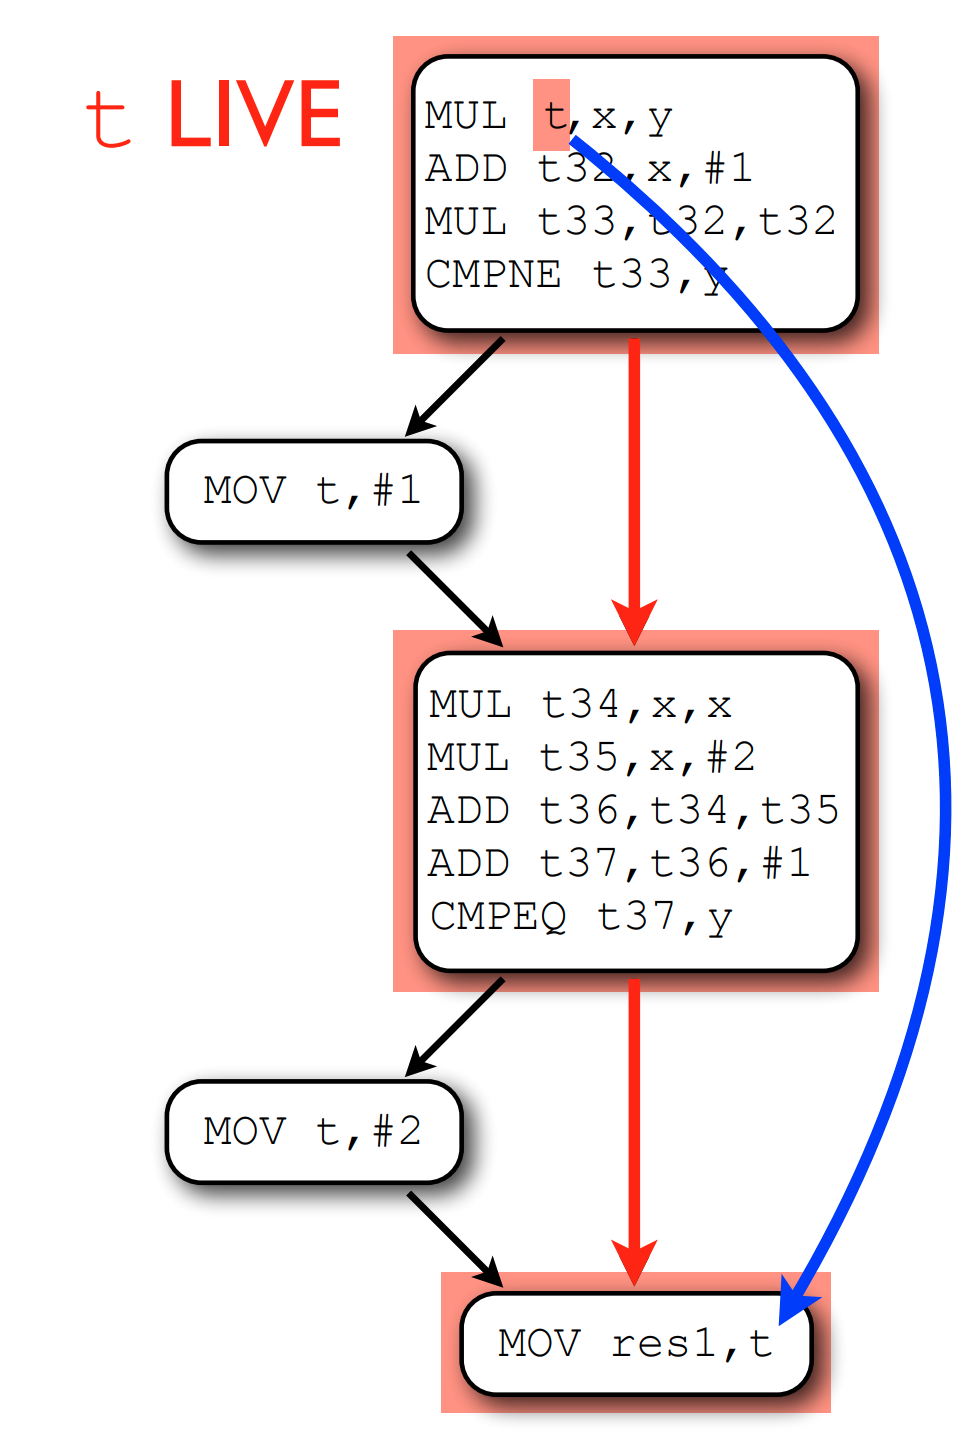
\includegraphics[width=0.3\textwidth]{liveex.png}
    \caption{CFG}
    \label{fig:liveex}
\end{figure}




